\section{Implementation} % Slå sammen implementasjon og design? enklere å snakke om et "tema" istedenfor å dele det opp

% design skal være hvordan vi designer systemet vårt, kinda litt som high-level usecase hvor vi beskriver hvordan ting skal virke for brukeren, mens design viser hvordan det ca skal sitte sammen logikk wise. Implementation skal være spesifikt hvordan vi har gjort det med kode, så må nesten være separate

This section will look closer into the ideas, code and structure behind various parts of the application. all shown code is written by the project group members. One important aspect of Unreal Engine to remember is that the order of axes might be different than other industry standards, as Unreal Engine uses a Left Handed, Z Up coordinate system. (source) In this three-dimensional space, the \textbf{X}-axis points forwards, the \textbf{Y}-axis points to the right, and the \textbf{Z}-axis points upwards. 

\subsection{Spline Tool}

One of the first goals specified by the client was to move the train along a straight path. Seeing as a later goal was to also implement curvature, we decided that it would be beneficial to begin work on curved train movement right away, as this would likely save us some time. In the existing simulator, the railway is procedurally generated from a list of points forming a \textit{spline}. A spline can be defined as a mathematical function to interpolate and form a smooth curve between multiple points. Each point is made up of a location vector and a tangent vector for specifying the curvature of the spline at the given position. We also looked into \textit{Bézier curves}, a similar alternative to splines, but Unreal Engine's built-in spline component made it an obvious choice. \newline

\begin{figure}[h]
    \centerline{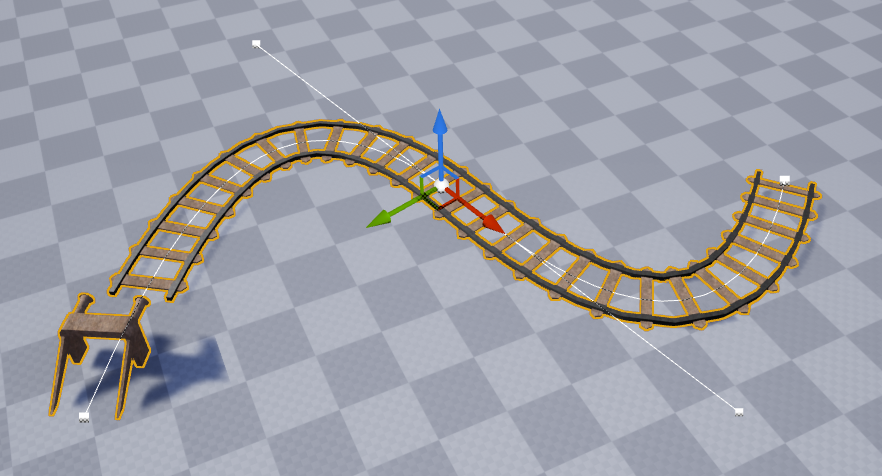
\includegraphics[width=0.9\textwidth]{figures/Spline1.png}}
    \caption[size=small]{A selected spline deforming a railway mesh along itself. The white squares indicate the spline points, and the white lines indicate the tangent of the selected spline point.}
\end{figure} 


We created \textit{ASplineActor}, a class for handling all functionality related to the railway. This class contains a \textit{USplineComponent}, a powerful component with functions for placing and deforming a mesh along a spline. In this context, a mesh can be described as a 3D-model. The way this initially works is by looping over all points in the spline, placing a sub-mesh that is stretched between points $P_n$ and $P_{n+1}$, and bending the meshes by the curvature of the tangents between $T_n$ and $T_{n+1}$. The spline points were defined by the user in the editor, and could be placed freely. The results looked promising, but a major flaw of this method occurs when any distances between each set of spline points aren't uniform. The meshes would stretch differently along the spline, making the railway look rather odd. A good analogy is imagining a skyscraper with a single, horizontally stretched window instead of separate windows on each floor. The solution to this was to split the spline into segments of equal length to that of the mesh/model itself, and add a new sub-mesh at each segment. Essentially cutting up the railway into pieces and replacing the existing spline points. The mesh used in figure \textbf{X} is a small slice of a railway created with primitive shapes in Asset Forge. \\

% CODE

% SKAL FJERNE MASSE AV KODEN DONT WORRY

\begin{code}

// Get the size vector of the mesh
const FVector MeshSize = Mesh->GetBoundingBox().GetSize();
	
// Get the length of the bounding box of the mesh along the forward axis
const float MeshLength = MeshSize.X;

...

const float SplineLength = SplineComponent->GetSplineLength();

// Set number of spline points to number of meshes fitting inside spline length
const int SplinePoints = FMath::CeilToInt(SplineLength / MeshLength);

for (int PointCount = 0; PointCount < SplinePoints; PointCount++)
{
	// Generate a spline mesh component for each point in the spline
	USplineMeshComponent* SplineMesh = 
	NewObject<USplineMeshComponent>(
	    this, USplineMeshComponent::StaticClass()
	);

	...
	
	// Get the location and tangents for the mesh at the 
	// current distance along the spline
	
	const float StartDistance = MeshLength * PointCount;
	
	FVector StartPoint = GetLocationAtDistanceAlongSpline(
	    StartDistance, ESplineCoordinateSpace::Local
    );
	    
	FVector StartTangent = GetDirectionAtDistanceAlongSpline(
	    StartDistance, ESplineCoordinateSpace::World
    );
    
	// Get the location and tangents for the end of the 
	// mesh at the current distance along the spline

	const float EndDistance = MeshLength * (PointCount + 1);
	
	FVector EndPoint = GetLocationAtDistanceAlongSpline(
	    EndDistance, ESplineCoordinateSpace::Local
	);
	
	FVector EndTangent = GetDirectionAtDistanceAlongSpline(
	    EndDistance, ESplineCoordinateSpace::World
	);
	
	...
	
	// Set the mesh location and curvature in spline
	SplineMesh->SetStartAndEnd(
	    StartPoint, 
	    StartTangent, 
	    EndPoint, 
	    EndTangent
    );
}
\end{code}
%\caption[size=small]{KODE! :D}

Opting for a custom spline class instead of Unreal Engine's solution let us change the spline into a railway, adding specific elements such as \textit{buffer stops}, the metal bars at the end of a railway to stop trains. We added an optional parameter to the ASplineActor class, where the user can input a separate mesh to be displayed as the first and/or the last sub-mesh of the spline. However, if this field is left empty, the sub-mesh will default to the given railway mesh. We also implemented a boolean flag which sets off if the spline extends a desired angle or curvature limit, to ensure the train looking natural when traversing the railway. \newline

\begin{figure}[h]
    \centerline{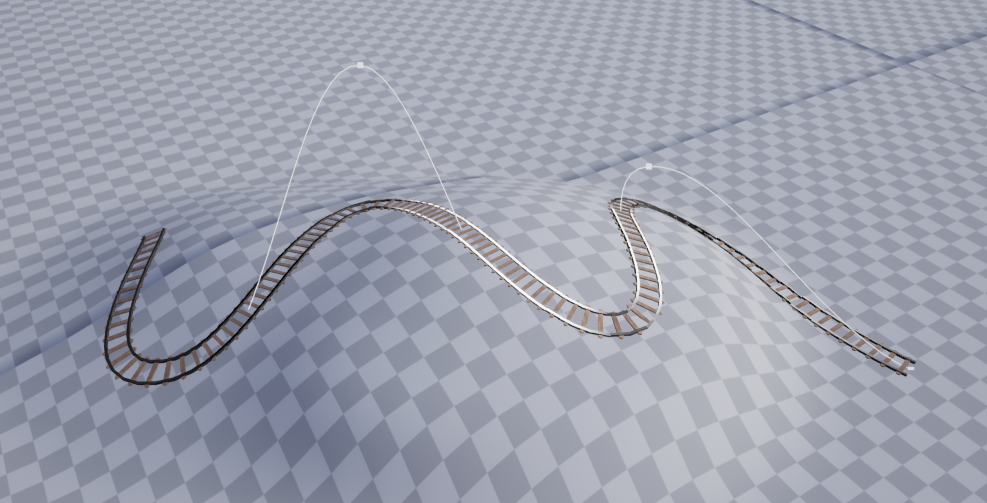
\includegraphics[width=0.9\textwidth]{figures/Spline2.png}}
    \caption[size=small]{A railway conforming to the terrain height}
\end{figure} 

One of the challenges with the tool occurred when manually placing the spline points. The railway curved naturally in the horizontal plane, but if the terrain had any difference in height, the railway would simply disappear under ground or hover above ground. To solve this, we perform a line cast in each spline point's X and Y coordinates, from the top to the bottom of the level. This is a way to see if we hit any terrain along the line cast. If there is a hit, the Z-coordinate of the relevant spline point is simply set to the height value of the terrain hit. This gets more computationally expensive the longer a spline is, but is only run once when a spline undergoes change, so any noticeable effects are minuscule. 
% kjør oppdatering av spline i en annen thread? da slipper editoren å lagge så mye når man endrer på ting. fant en plugin som bruker spline greier i en annen thread, men koster penger. Skal gå ann å lage en ny thread, gjøre computations der og sende det tilbake i game thread. - EH

\subsection{Signal controller}

The Central Signal Controller is responsible for signal and status communication between the signals and trains. The controller receives signal and status updates from TriggerBoxes, which are placed along the railway and are used to send signal or status updates depending on configured conditions. 

When the level is loaded and the game begins, the Central Signal Controller searches for all actors inheriting from the Basic Signal class. Valid actors are then sorted into lists based on which type they are, such as Main Signal or Forward Signal. These different lists are then used later to send signal updates. 

% vis kode som søker etter og lagrer actors fra central signal controller
\begin{code} 
void ACentralSignalController::FindAllSignals()
{
	// Finds all actors of signal classes
	UGameplayStatics::GetAllActorsOfClass(GetWorld(), DwarfSignalBP, DwarfSignalActors);
	UGameplayStatics::GetAllActorsOfClass(GetWorld(), MainSignalBP, MainSignalActors);
	UGameplayStatics::GetAllActorsOfClass(GetWorld(), ForwardSignalBP, ForwardSignalActors);

	int32 i = 1;

	// Loops through all actors
	for (AActor* DwarfSignalActor : DwarfSignalActors)
	{
		ABasicSignal* DwarfSignal = Cast<ABasicSignal>(DwarfSignalActor);
		if (DwarfSignal)
		{
			FString TagName = FString::Printf(TEXT("Dwarf_%i"), i++);
			
			DwarfSignal->Tags.Add(FName(TagName));

			AllSignalActors.Add(DwarfSignalActor);
		}
	}
	...
}
\end{code}

When the controller receives a signal update, an ID, new signal state and signal type must be specified. The controller then searches through the specified signal list to match the IDs, and when this happens the new signal state is sent. The controller continues searching the list, if more than one signal shares the same ID. Given that the length of the list of signals is quite short, the time spent searching the list even when the first match is found is insignificant. % measure this? or at least prove the time spent will have a small to none effect on fps

% vis kode som finner riktig signal og sender signalet
\begin{code}
void ACentralSignalController::SendUpdatedSignal(FName SignalID, ESignalType SignalType, ESignalStatus Status)
{
	TArray<AActor*> Actors;

	// Selects relevant actors to search based on signal type
	switch (SignalType)
	{
	case ESignalType::Main:
		Actors = MainSignalActors;
		break;
	case ESignalType::Forward:
		Actors = ForwardSignalActors;
		break;
	case ESignalType::Dwarf:
		Actors = DwarfSignalActors;
		break;
	default:
		checkNoEntry();
		break;
	}

	// Loops through all signals
	for (AActor* SignalActor : Actors)
	{
		ABasicSignal* Signal = Cast<ABasicSignal>(SignalActor);
		if (Signal && (Signal->ID == SignalID))
		{
			// If the signal matches the incoming id, update the status
			Signal->UpdateSignalStatus(Status);
		}
	}
}
\end{code}

As the Central Signal Controller is an actor, it needs to be placed in every level which is going to use signals. One alternative would be to create a subsystem with the same functionality. This would allow the controller to work in any level without needing to place an actor, as well as having a more predictable and stable lifecycle. 

\subsection{Signals}

The class ABasicSignal is used for the three different types of signals. The three signal types share the same functionality, with the only difference being the models used and number of lights on each model, as well as which colors are used and how the signal reacts to signal status updates. 

% vise bilde av blueprint kode som bestemmer signal status greier

different models have different numbers and locations, so automatic light creation and placement is used

dynamic signal creation at runtime, uses sockets to place signal lights, emissive lights used

% vise kode som lager lysene på signalene
\begin{code}
void ABasicSignal::SetupLight()
{
	RemoveLights();

	// Create all lights in a loop
	for (int32 i = 0; i < NumLights; i++)
	{
		FString SocketName = FString::Printf(TEXT("Socket_%i"), i + 1);
		FString LightMeshName = FString::Printf(TEXT("LightMesh_%i"), i + 1);

		UStaticMeshComponent* LightMesh = NewObject<UStaticMeshComponent>(this, FName(LightMeshName));

		// Creates a new light struct
		FSignalLight NewLight(LightMesh);

		NewLight.LightMesh->SetStaticMesh(BaseLightMesh);

		NewLight.LightMesh->SetupAttachment(VisualComponent, FName(SocketName));

		// Creates the instanced dynamic light material
		NewLight.DynMaterial = UMaterialInstanceDynamic::Create(BaseLightMaterial, this);

		NewLight.DynMaterial->SetScalarParameterValue("Emissive_Strength", MaxLightLevel);
		NewLight.DynMaterial->SetVectorParameterValue("Emissive_Color", FLinearColor(1.0f, 1.0f, 1.0f));

		NewLight.LightMesh->SetMaterial(0, NewLight.DynMaterial);

		NewLight.LightMesh->RegisterComponent();


		Lights.Add(NewLight);
	}
}
\end{code}

registers new component, otherwise the object is garbage collected

creates a new dynamic material instance to give each light its own color and properties

\subsection{Editor Mode}
The goal of the editor mode was to give the client a simple tool build worlds and train scenarios. Our task was to implement the ability to place, move and rotate objects such as trains and buildings, and a way to lay a railway across the terrain. We decided to design this tool based on the tools available in Unreal Engine's own editor, as these would accomplish similar tasks. For moving objects around, we created a \textit{gizmo} consisting of one arrow for each axis, and a square for the plane along the X- and Y-axes. Once an object is selected, this gizmo appears at its position, utilizing custom depth rendering, which enables the gizmo to always be visible even when it is covered by another mesh. 

\begin{figure}[h]
\centering
\begin{minipage}{.5\textwidth}
  \centering
  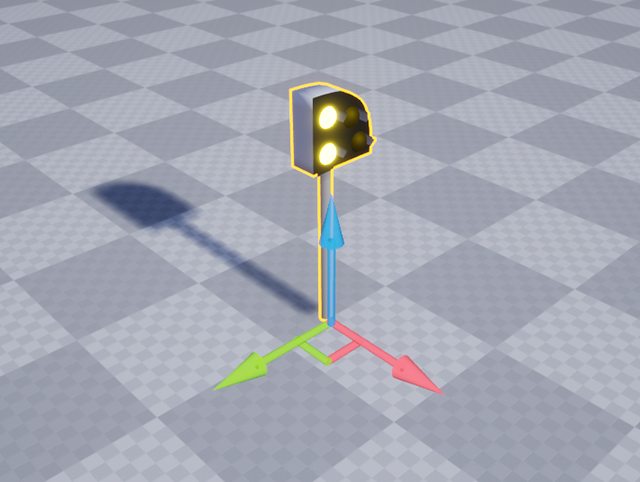
\includegraphics[width=0.95\linewidth]{figures/Gizmo1.png}
  \captionof{figure}{The translation gizmo on a selected signal}
  \label{fig:test1}
\end{minipage}%
\begin{minipage}{.5\textwidth}
  \centering
  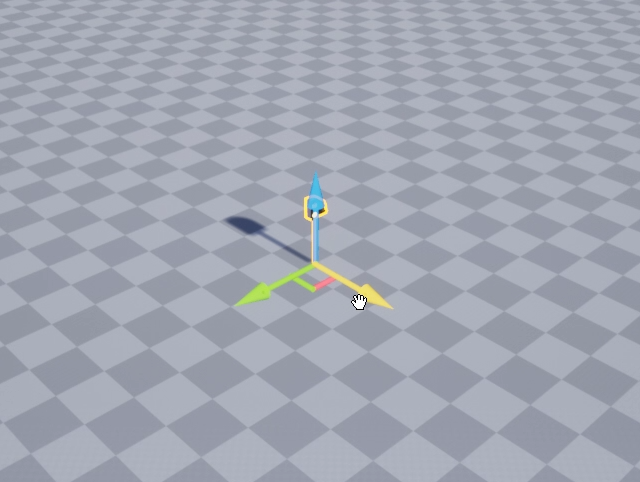
\includegraphics[width=0.95\linewidth]{figures/Gizmo2.png}
  \captionof{figure}{The translation gizmo far away, hovering the X-axis arrow}
  \label{fig:test2}
\end{minipage}
\end{figure}

By hovering the mouse over one of the gizmo's arrows and dragging, the user can move the object in the relevant axis. This is done by casting a line from the camera, in the direction of the cursor's position on the screen, and processing the results on hit. This is done in a separate collision layer for gizmos, such that the line is not obscured by any object. The tool includes two modes, translation and rotation. When switching mode to rotation, the arrow meshes are replaced by a cogwheel in the X-Y axis plane, which rotates the object around the Z axis when dragged. These gizmos are made to be a part of the user interface, and get scaled based on their distance from the camera to keep their size uniform. 

When grabbing a gizmo arrow to move an object, the position of the cursor is saved as a variable in the first frame of holding down the mouse button. This position is used to get the offset between the gizmos center position (also the object anchor position), and the cursor. While dragging the gizmo arrow, the objects position is set to the location of the cursor minus the offset, resulting in the object moving in parallel with the cursor. This behaviour works fine in theory, but during testing, we found a lack of user friendliness due to the cursor having to overlap the gizmo during dragging. To combat this, we added secondary meshes to each arrow that would inflate the area of interaction. These meshes were given an invisible material, so the user could not see them, but were able to interact with them.

\begin{figure}[h]
\centering
\begin{minipage}{.5\textwidth}
  \centering
  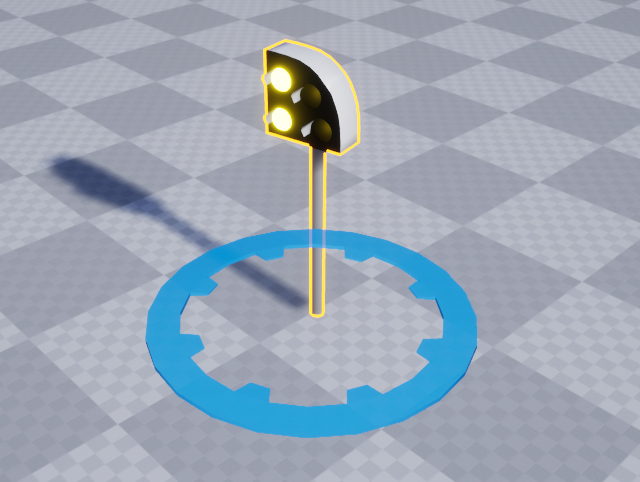
\includegraphics[width=0.95\linewidth]{figures/Gizmo3.png}
  \captionof{figure}{The rotation gizmo in the X-Y plane}
  \label{fig:test1}
\end{minipage}%
\begin{minipage}{.5\textwidth}
  \centering
  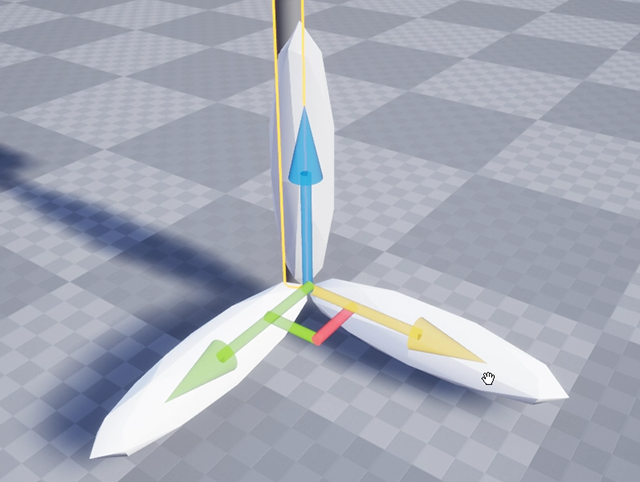
\includegraphics[width=0.95\linewidth]{figures/Gizmo4.png}
  \captionof{figure}{Additional meshes around the arrows}
  \label{fig:test2}
\end{minipage}
\end{figure}

During user testing with the client, it was made clear that this interaction was still hard, as the cursor would, more often that not, exit the area of these meshes. This was towards the very end of the development, and there was not enough time to iterate on this implementation, as it would quickly grow complicated. But due to the curious nature of programmer brains, we were attracted towards finding a solution to this problem. Even if we did not have the time to finish the implementation of these ideas, we came up with several possible solution that could fix or recreate this system entirely.

The first idea was to 